\documentclass[7pt]{article}
\twocolumn
\usepackage[utf8]{inputenc}
\usepackage{graphicx}
\usepackage{subcaption}
\usepackage{caption}
\usepackage{siunitx}
\usepackage{hyperref}
\graphicspath{{./images/}}
\usepackage{amsmath}

\usepackage{natbib}
\bibliographystyle{abbrv}
\usepackage[superscript,biblabel]{cite}

\usepackage[a4paper, total={183mm, 247mm}]{geometry}
\usepackage[left]{lineno}
% \linenumbers

\newcommand*{\ts}{{\tau^{*}}}
\newcommand*{\diff}{\mathop{}\!\mathrm{d}}
\newcommand{\ps}{\si{\pico\second}}
\newcommand{\ns}{\si{\nano\second}}
\newcommand{\fs}{\si{\femto\second}}
\newcommand{\ips}{\si{\per\pico\second}}
\newcommand{\us}{\si{\micro\second}} 
\newcommand{\iA}{\si{\per\angstrom}}
\newcommand{\K}{\si{\kelvin}} 

\usepackage{sectsty}
\sectionfont{\small}

\title{Reductionism, surface dynamics and the Kramers problem}

\author{Jeremy Wilkinson}
\date{September 2021}

\begin{document}

\maketitle

The development of experimental methods such as Helium Spin-Echo Microscopy marked a revolution in the ability to observe the diffusion of adatoms over a substrate\cite{FouquetHSEM, JardineHSEM}. While the observables in a surface scattering experiment contain a full statistical description of adatom motion\cite{vanHowe}, the microscopic trajectories of adatoms are not directly observable. The nature of microscopic adatom motion from which macroscopic observable quantities emerge therefore remains open to conjecture. As is often the case with large thermodynamic systems, the details of the vast majority of degrees of freedom in the system are irrelevant to the quantities of interest. Very little can be known about the exact state of a substrate and its interactions with an adsorbate, and yet physical properties emerge which can be reliably defined and measured with complete ignorance to the vast majority of information in the system. The questions therefore arise, \emph{what are the observable quantities in a system} and \emph{what is the minimum amount of information one needs to know to explain these observables}. 

In the case of surface diffusion at low temperatures, one finds that adatoms are predominantly bound to local minima in the substrate potential, reffered to as adsorbtion sites. As an adatom oscillates about its local adsorbtion site it is able to slowly exchange energy with the substrate through interactions with surface phonons. On occasion, the adatom will find itself with enough energy to overcome the trapping potential and is able to hop to an adjacent site, or further. The hopping rate is therefore determined by the shape of the trapping well, in particular the activation energy, as well as the rate at which the adatom exchanges energy with the substrate.

While it is relatively simple to extract an activation energy directly from experimental data\cite{someone}, it is not possible to disentangle the energy exchange rate of the system from other effects without making further assumptions. The most common approach is to assume that the force on the particle may be treated as a random variable obeying the Markovian Langevin equation,
\begin{equation}
\begin{gathered}
	m\ddot{\vec{r}}=-m\eta\dot{\vec{r}}-\nabla U(\vec{r})+\vec{f}(t) \\ 
	\text{ where } \left<f(t_1)f(t_2)\right>=2k_BTm\eta\delta(t_1-t_2),
\end{gathered}
	\label{eq:langevin}
\end{equation}
and to fit the experimental data with simulated solutions to the Langevin equation. The resulting best fit friction parameter, $\eta$, parametrizes the strength of the random force $\vec{f}$ and may be used as a quantifier of the rate of energy transfer with the substrate.

Implicit to the construction of the Markovian Langevin equation is the assumption that the random force $\vec{f}(t)$ is uncorrelated in time. In the Fourier domain, this requirement translates to a uniform power spectrum $\left<\tilde{f}(\omega_1)\tilde{f}(\omega_2)\right>=4\pi k_BTm\eta\delta(\omega_1+\omega_2)$. However, the source of the noise in a surface dynamics system, the substrate phonons, have a well defined cutoff frequency and therefore the force they exert must be correlated in time. The effect of these noise correlations was previously ignored and assumed to be negligable. 

Through theoretical and computational study, the work presented here demonstrates that noise correlations can in fact have a significant effect on a system's energy exchange rate and thereby the long-time observables, such as the hopping rate. We also present (hopefully) a simple mechanism to estimate whether the noise cutoff has a large effect on a given system or whether it may be safely neglected. Finally we demonstrate why the use of the Markovian Langevin equation has nevertheless been succesful and thereby conclude that the energy exchange rate, defined as the correlation time of the total energy auto-correlation function is in fact a fundamental parameter in the determination of hopping. 

\section*{Energy exchange and hopping rates}

The energy exchange rate is an important quantity in the determination of hopping rates because it controls the number of independent energy levels the adatom attains per unit time. The fraction of time spent above the activation energy is set by Boltzmann statistics, however the \emph{number of times} this energy level is attained is set by the energy exchange rate. For this reason, we define the energy exchange rate as the inverse of the correlation time, $\phi$, of the \emph{total energy} autocorrelation function, $$\frac{\left<E(t)E(0)\right> - \left<E\right>^2}{\left<E^2\right> - \left<E\right>^2},$$ as shown in Fig. \ref{fig:e_auto}. In cases where an exponential could not be fit to the autocorrelation function, $\tau$ was taken to be the interval over which the autocorrelation function decays by a factor of $1/e$. For a Markovian Langevin equation in the presence of a harmonic potential, the energy exchange rate is given precisely by $\eta$, however in general this is not the case.


The observable quantity in a surface scattering experiment is the intermediate scattering function,
$$
\mathrm{ISF}(\Delta{\vec{K}}, t) = \left<\exp\left(i\Delta{\vec{K}}\cdot\vec{r(t)}\right)\right>.
$$
Typically the ISF is quoted for a single momentum transfer, $\Delta{K}$, over a range of time, as shown in the main axes of Figure \ref{fig:isf_dk}. For the purposes of extracting long-time transport co-efficients (read average rate of diffusion over the surface), the exponential decay rate of the ISF at long times, $\Gamma(\Delta{\vec{K}})$, is the quantity of interest and is proportional to the hopping rate\cite{Chudley}. By varying the magnitude of $\Delta{K}$ in a particular direction, one may calculate the jump distribution plot as shown in the inset of Figure \ref{fig:isf_dk}. When an adatom escapes from a well, it may hop more than one site before it settles down again. The spectral content, and therefore the shape, of the jump distribution is set by the relative probability of the number of sites an adatom travels before settling down again. The Markovian Langevin equation has been succesfully used to fit both the overal jump rate and jump distributions of physics systems \cite{Alexandrowicz, Hedgeland, Jardine} and non-stochastic molecular dynamics simulations \cite{Diamant}. 

The effects of noise correlations on the energy decorrelation rate were evaluated using the generalised Langevin equation,
\begin{equation}
	m\ddot{\vec{r}}+m\eta\int_0^t\diff{t'}K(t-t')\dot{\vec{r}}(t')+\nabla U(\vec{r})=\int_0^t\diff{t'}\vec{f}(t')K(t-t'),
	\label{eq:gle}
\end{equation}
with an exponential memory kernel, $K(t)=\exp(-\frac{t}{\tau})$, parametrized by the noise correlation time $\tau$. The resulting noise has a Lorentzian power spectrum given by $\left|\tilde{K}(\omega)\right|^2=\frac{1}{1+\omega^2\tau^2}$ with a half-width at half-maximum given by $\omega_c = \frac{1}{\tau}$.

Fig. \ref{fig:eta_tau_ttf_gamma} shows the energy exchange rate and ISF dephasing rate of the simulation over a range of $\eta$ and $\tau$ values. The top left panel demonstrates that regardless of the value of $\tau$, the energy exchange rate is proportional to $\eta$, although the gradient of the line  $\tau$

\begin{figure*}
	\centering
	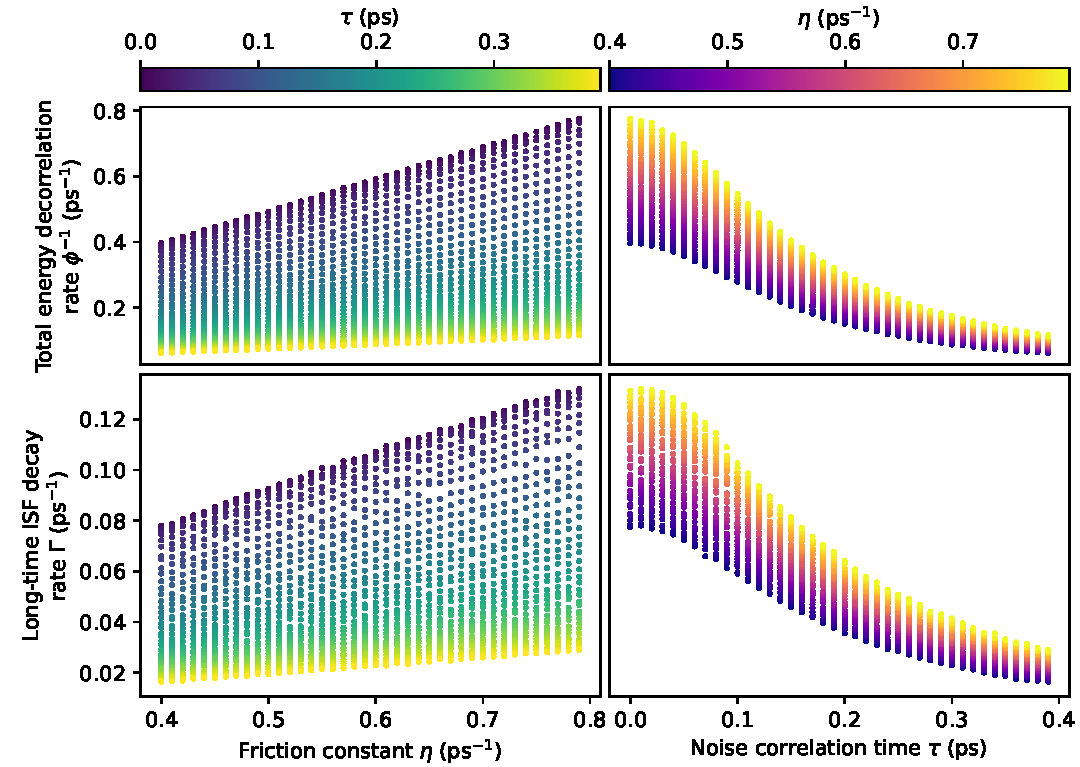
\includegraphics[width=1.0\textwidth]{eta_tau_ttf_gamma}
	\caption{}
	\label{fig:eta_tau_ttf_gamma}
\end{figure*}

 we present the results of  
\begin{figure}
	\centering
	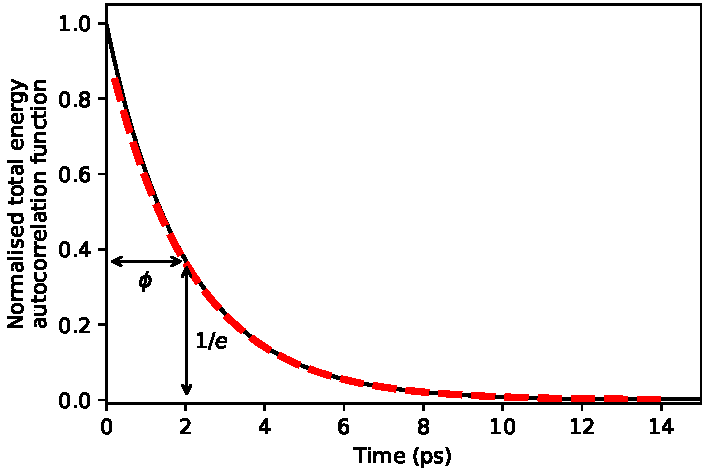
\includegraphics[width=1.0\columnwidth]{e_auto}
	\caption{}
	\label{fig:e_auto}
\end{figure}

\section*{The inertial cutoff}

\section*{Non-linear friction}

\section*{Discussion and outlook}

simple to extract from experThe most common method of quantifying the energy exchange rate with the substrate is to fit experimental data with a Markovian Langevin simulation in which the force of the adatom at any instant is assumed to be of the form 



This activated diffusion process is characterized through the rate at which adatoms hop between adsorbtion sites as well as the distribution of the distances hopped before the adatoms settle down into the next adsorbtion site. 

Hopping rate are observed to follow an Ahrrenius law\cite{someone}, $$\gamma=A\exp(-E_a/kT),$$ parametrized by an activation energy $E_a$ and a pre-exponential factor, $A$, carrying units of inverse time, usually assumed to be temperature independent. The Boltzmann factor may be understood as quantifying the probability of the particle having enough energy to overcome the barrier, and the prefactor contains the rate at which this energy level is attained and the probability of a hop occuring when sufficient energy is attained.



For an adatom weakly coupled to substrate phonons, the Ahrrenius law can be understood as the product of the rate at which the particle changes its energy, the probability of the particle finding itself with enough energy to overcome the activation barrier and the probability  

The Markovian Langevin equation, 
\begin{equation}
	m\ddot{\vec{r}}+m\eta\dot{\vec{r}}+\nabla U(\vec{r})=\vec{f}(t) \text{ where } \left<f(t_1)f(t_2)\right>=2k_BTm\eta\delta(t_1-t_2),
	\label{eq:langevin}
\end{equation}
provides such a simplification for the trajectory, $\vec{r}(t)$, of a single `tagged' particle coupled to a heatbath\cite{Kramers}. The inherently chaotic interactions with the heatbath's degrees of freedom are summarized through a random noise force $f$ and a friction term, the strength of which is parametrized by a single parameter $\eta$. The equilibrium statistical physics of this equation is well understood with an equilibrium phase space density function given by $\rho(\vec{r}, \vec{p})=\frac{1}{\mathcal{Z}}\exp\left(-H(\vec{r}, \vec{p})/kT\right)$ exactly\cite{Zwanzig}.

While analytically tractable, the Markovian approximation neglects correlations in the random force present in all physical systems. The Langevin equation can be modified to include noise correlations through convolution with a memory kernel $K(t)$, with a corresponding modification to the friction term required to preserve equipartition of energy \cite{Kubo}. The resulting generalised Langevin equation, 
\begin{equation}
	m\ddot{\vec{r}}+m\eta\int\diff{t'}K(t-t')\dot{\vec{r}}(t')+\nabla U(\vec{r})=\int\diff{t'}\vec{f}(t')K(t-t'),
	\label{eq:gle}
\end{equation}
captures linear correlations in noise with a power spectrum given by the power spectrum of $K$. For a non-zero background potential, $U(\vec{r})$, the fluctuation dissipation theorem (the second condition of Equation \ref{eq:langevin}), is not enough to gaurentee exact equipartition of energy. Fortunately, it remains a very good approximation for a kernel with a total area of $1$ though it is not hard to construct a situation where the equipartition theorem is violated (see supplemental material). 


Analytic expressions for the escape rate, $\gamma$, of a Markovian Langevin particle from a trapping well of natural frequency $\omega_0$ in the low friction, $\frac{\eta}{\omega_0} < 1$, regime explain the Ahrrenius nature of hopping rates seen in experimental and computational studies. 

Although the results in this paper demonstrate that noise correlations can have a significant effect on the hopping rate, the reason why the Markovian Langevin has seen success regardless of this will also become clear.

Something about energy exchange rates \& hopping rates
Something about activated diffusion being bound with occasional hops

\begin{figure}
	\centering
	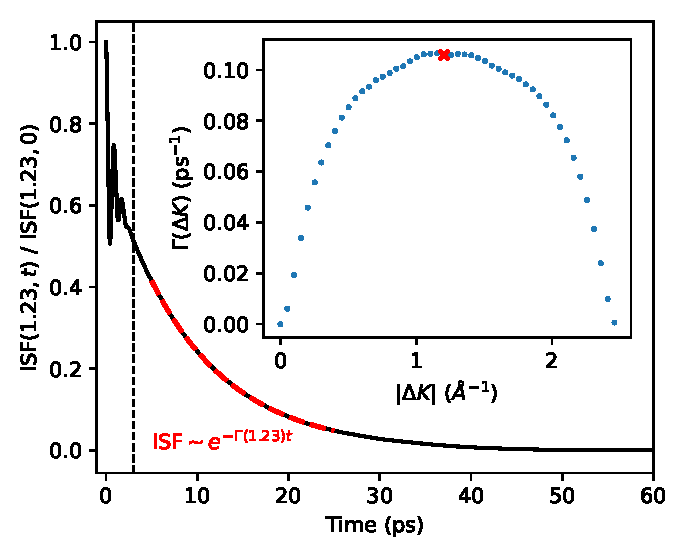
\includegraphics{isf_dk}
	\caption{}
	\label{fig:isf_dk}
\end{figure}

\section{Computational Model}

A simulation was constructed to solve the non-Markovian Langevin equation with an exponential memory kernel $K(t)=\frac{1}{\tau}\exp(-t/\tau)$ using a timestep of $1\fs$. The 2D background potential was extracted from a molecular dynamics model of Sodium adsorbed on Copper(001) by calculating the free energy, $U(\vec{x}) = - kT \log(\left< \delta(\vec{r}(t)-\vec{x}) \right>)$, from a series of trajectories totalling $2 \us$ of run time. The resulting $100\times100$ potential grid, shown in Figure \ref{pot_surface},  covering the unit cell was interpolated through a bicubic spline\cite{press1992numerical} and used to tile the plane. At each timestep of the Langevin simulation, the force on the particle was calculated from the gradient of the interpolated potential grid and added to the friction and noise force convolved with the memory kernel using the relation,
$$
\int_0^{n\Delta{t}} dt' K\left(t-t'\right) \vec{f}(t') \approx \alpha \int_0^{(n-1)\Delta{t}} dt' K\left(t-t'\right) \vec{f}(t') + \frac{1}{1-\alpha} \vec{f}\left(t_n\right)
$$
with $\alpha=\exp(-\frac{\Delta{t}}{\tau})$.

\begin{figure}
	\centering
	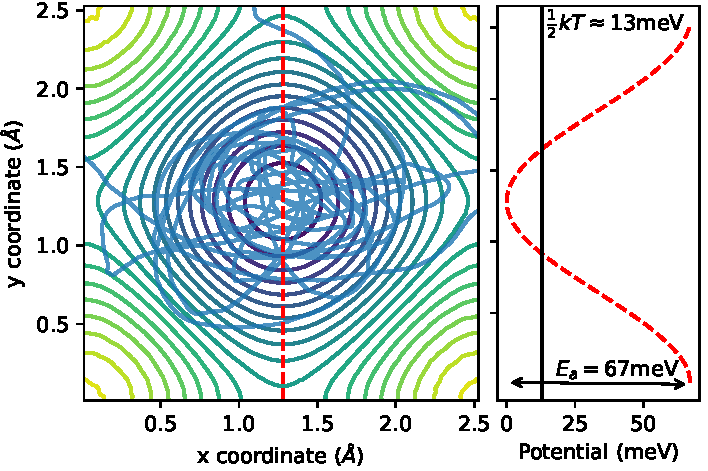
\includegraphics{pot_surface}
	\caption{}
	\label{pot_surface}
\end{figure}

\bibliography{bibliography}

\end{document} 
